\documentclass{standalone}
\usepackage{tikz}
\usetikzlibrary{automata, positioning, arrows}

\begin{document}
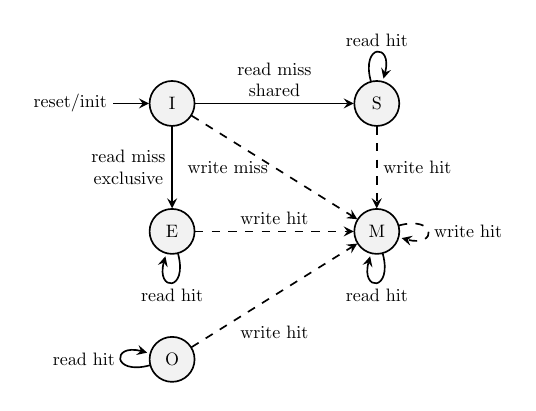
\begin{tikzpicture}[node distance=2.5cm,initial text={reset/init}]
\tikzstyle{every node}=[scale=0.65]
\tikzstyle{every state}=[semithick, fill=gray!10]
\tikzstyle{every edge}=[draw,->,>=stealth,auto,semithick]

\node[state, initial] (I) {I};
\node[state,below of=I] (E) {E};
\node[state,right of=E,node distance=4cm] (M) {M};
\node[state,right of=I,node distance=4cm] (S) {S};
\node[state,below of=E] (O) {O};

\draw (M) edge[loop below] node {read hit} (M)
            edge[loop right, dashed] node {write hit} (M);
\draw (I) edge[dashed] node[left] {write miss} (M)
            edge node[align=center,above] {read miss\\shared} (S)
            edge node[align=center,left] {read miss\\exclusive} (E);
\draw (S) edge[dashed] node {write hit} (M)
            edge[loop above] node {read hit} (S);
\draw (E) edge[dashed] node {write hit} (M)
            edge[loop below] node {read hit} (E);
\draw (O) edge[loop left] node {read hit} (O)
            edge[dashed] node[below=0.3cm] {write hit} (M);
\end{tikzpicture}
\end{document}
